%!TEX root = vorlage.tex

\subsection{Quality measures for evaluation}%
\label{subsec:quality-measures}%
A performance measure is a crucial part of any machine learning system, but
there are other measures of quality which matter when segmentation algorithms
are compared. This section gives an overview of those quality measures.


\subsubsection{Accuracy}
Showing the correctness of the segmentation hypotheses is done in most
publications about semantic segmentation. However, there are a couple of
different ways how this accuracy can be displayed. One way to give readers a
first impression of the obtained segmentations is by showing examples such
as~\cref{fig:segmentation-example}.

\begin{figure}
\centering
\subfigure[Example Scene \label{fig:segmentation-example-scene}]{
  
\includegraphics[width=0.45\linewidth, keepaspectratio]{figures/image-segmentation-example.jpg}
}%
\subfigure[Visualization of a found segmentation \label{fig:segmentation-example-seg}]{
  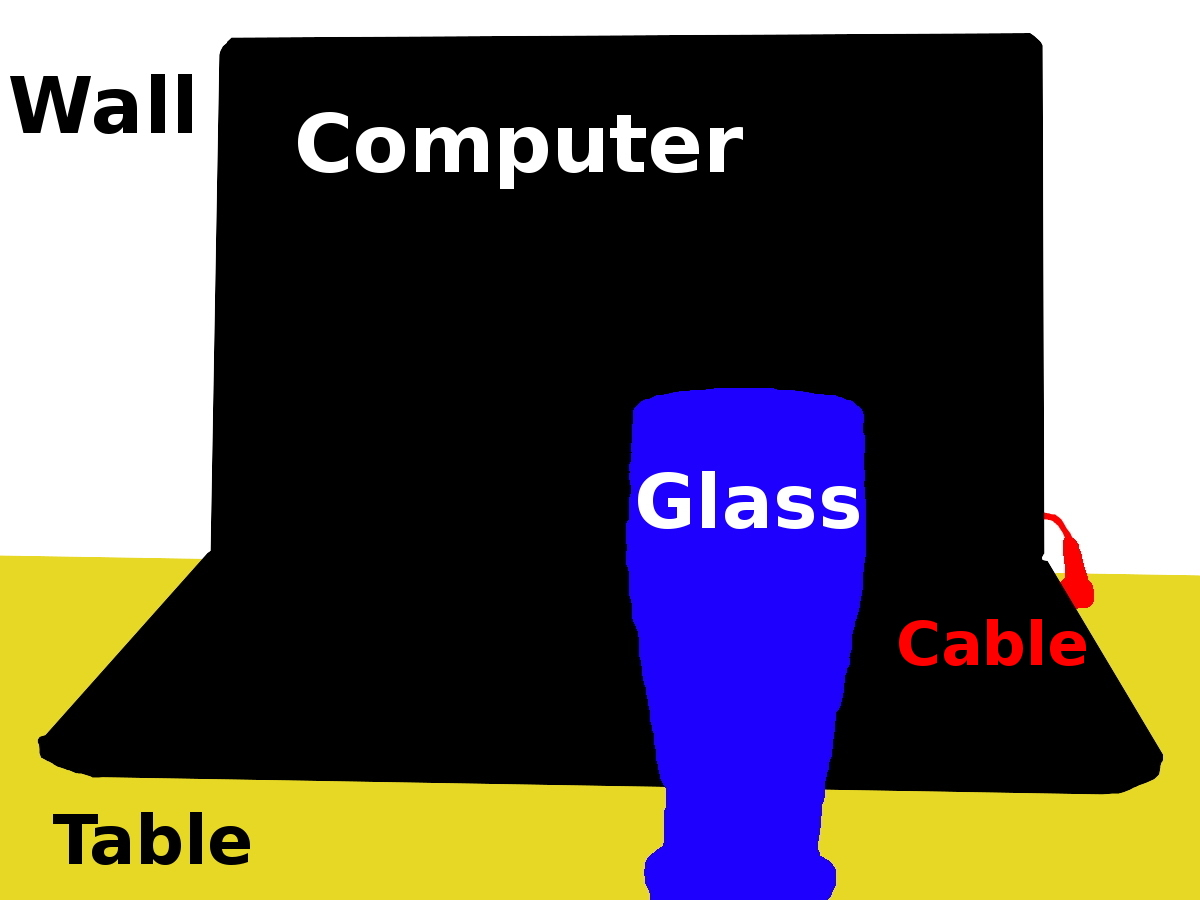
\includegraphics[width=0.45\linewidth, keepaspectratio]{figures/image-segmentation-example-segmented.jpg}
}
\caption{An example of a scene and a possible visualization of a found segmentation.}
\label{fig:segmentation-example}
\end{figure}

However, this can only support the explanation of particular problems or
showcase special situation. For meaningful information about the overall
accuracy, there are a couple of metrics.

For this section, let $k \in \mathbb{N}$ be the number of classes, $n_{ij} \in
\mathbb{N}_0$ with $i,j \in 1, \dots, k$ be the number of pixels which belong to
class~$i$ and were labeled as class~$j$. Let $t_i = \sum_{j=1}^k n_{ij}$ be the
total number of pixels of class~$i$.

One way to compare segmentation algorithms is by the pixel-wise accuracy of the
predicted segmentation as done in many publications
\cite{shotton2006textonboost,csurka2008simple,long2014fully}. This is also
called per-pixel rate and defined as $\frac{\sum_{i=1}^k n_{ii}}{\sum_{i=1}^k
t_i}$. Taking the pixel-wise classification accuracy has two major drawbacks:

\begin{problemnr}
    \item \label{item:problem-large-regions} Tasks like segmenting images for
          autonomous cars have large regions which have one class. This makes
          achieving classification accuracies of more than \SI{30}{\percent}
          with a priori knowledge only possible.
    \item \label{item:problem-labeling-granularity} The manually labeled images
          could have a more coarse labeling. For example, a human classifier
          could have labeled a region as
          \enquote{car} and the algorithm could have split that region into
          the general \enquote{car} and the more specific \enquote{wheel of a
          car}
\end{problemnr}
\goodbreak
Three accuracy metrics which do not suffer from
\cref{item:problem-large-regions} are used in~\cite{long2014fully}:\nobreak%
\begin{itemize}
    \item \textit{mean accuracy}: $\frac{1}{k} \cdot \sum_{i=1}^n \frac{n_{ii}}{t_i}$
    \item \textit{mean intersection over union}: \hfill\\$\frac{1}{k} \cdot \sum_{i=1}^k \frac{n_{ii}}{t_i + \sum_{j=1}^k n_{ji}-n_{ii}}$
    \item \textit{frequency weighted intersection over union}:
          ${({\sum_{p=1}^k t_p})}^{-1} \sum_i \frac{t_i n_{ii}}{t_i + \sum_{j=1}^k n_{ji} - n_{ii}}$
\end{itemize}

Another problem might be pixels which cannot be assigned one of the known
classes. For this reason, \cite{shotton2006textonboost} makes use of a void
class. This class gets completely ignored for all quality measures. Hence the
total number of pixels is assumed to be $\text{width} \cdot \text{height} - \text{number of void pixels}$.

One way to deal with \cref{item:problem-large-regions} and
\cref{item:problem-labeling-granularity} is giving a \textit{confusion matrix}
as done in \cite{shotton2006textonboost}. However, this approach is not
feasible if many classes are given.

The $F$-measure is useful for binary classification task such as the KITTI road
segmentation benchmark~\cite{Fritsch2013ITSC} or crypt segmentation as done
by~\cite{cohen2015memory}. It is calculated as \enquote{the harmonic mean of
the precision and recall}~\cite{pantofaru2005comparison}:
\[F_\beta = (1+\beta)^2 \frac{\text{tp}}{(1+\beta^2)\cdot \text{tp}+ \beta^2 \cdot \text{fn} + \text{fp}}\]
where $\beta=1$ is chosen in most cases and \texttt{tp} means \textit{true
positive}, \texttt{fn} means \textit{false negative} and  \texttt{fp} means
\textit{false positive}.

Finally, it should be noted that a lot of other measures for the accuracy of
segmentations were proposed for non-semantic segmentation. One of those
accuracy measures is \textit{Normalized Probabilistic Rand}~(NPR) index which
was introduced in \cite{unnikrishnan2005measure} and evaluated
in~\cite{celebi2009improved} on dermoscopy images. Other non-semantic
segmentation measures were introduced in~\cite{martin2001database}, but the
reason for creating them seems to be to deal with the under-defined task
description of non-semantic segmentation. These accuracy measures try to deal
with different levels of coarsity of the segmentation. This is much less of a
problem in semantic segmentation and thus those measures are not explained
here.


\subsubsection{Speed}%
\label{subsubsec:speed-quality-measure}%
A maximum upper bound on the execution time for the inference on a single image
is a hard requirement for some applications. For example, in the case of
autonomous cars an algorithm which classifies pixel as street or no-street
and thus makes a semantic segmentation, every image needs to be processed
within \SI{20}{\milli\second}~\cite{bittel2015pixel}.

Most papers do not give exact values for the time their application needs. One
reason might be that this is very hardware, implementation and in some cases
even data specific. For example, \cite{hoover1996experimental} notes that their
algorithm needs \SI{10}{\second} on a Sun SparcStation~20. The fastest CPU ever
produced for this system had~\SI{200}{\mega\hertz}. Comparing this directly
with results which were obtained using an Intel~i7-4820K with
\SI{3.9}{\giga\hertz} would not be meaningful.

However, it does still make sense to mention the execution time as well as the
hardware in individual papers. This gives the interested reader the possibility
to estimate how difficult it might be to adjust the algorithm to work in the
required time-constraints. Also, it should be noted if the algorithm can be
executed in parallel as standard \glspl{GPU} on the consumer market can execute
up to 256~kernels in parallel.


\subsubsection{Stability}%
\label{subsubsec:stability-quality-measure}%
The stability of segmentation is a desirable quality measure. One the one hand,
there are some variants of images like slight blurring, Gaussian noise and
similar which should not change the segmentation at all. Also, two images which
show a slight change in perspective should also only result in slight changes
in the segmentation~\cite{pantofaru2005comparison}.

Another desirable stability criterion is parameter choice. If the
segmentation algorithm has hyperparameters, then slightly changing those should
also only result in minor differences of the resulting
segmentations~\cite{pantofaru2005comparison}.


\subsubsection{Memory usage}
Peak memory usage matters when segmentation algorithms get used in devices like
smartphones or cameras, or when the algorithms have to finish in a given time
frame, run on the \gls{GPU} and consume so much memory for single image
segmentation that only the latest graphic cards can be used. However, no
publication we found mentioned the peak memory usage.
